\subsection{Architettura del Ranking Service}
\subsubsection{Descrizione}
Il microservizio denominato \textit{Ranking Service} si occupa principalmente di due funzionalità:
\begin{itemize}
    \item Crawling dei dati: questo processo avviene tramite l'utilizzo della libreria Instagrapi. Ogni volta che viene chiamato il metodo start\_crawling della classe FacadeCrawling, il sistema sceglie dal proprio database il profilo Instagram che non viene guardato da più tempo e ne effettua il crawling dei dati. Per ogni media prelevato dal profilo, viene analizzata la sua location e nel caso in cui essa sia quella di un ristorante, il media viene salvato nel database ed inviato alla coda SQS in modo che possa essere analizzato dal servizio \textit{Ranking Service};
    \item Suggerimento dei profili: questa funzionalità viene esposta tramite una API rest al frontend al fine di fornire all'utente la possibilità di suggerire un profilo instagram sul quale successivamente il sistema andrà ad effettuare il crawling dei dati. Prima di essere aggiunto al database, viene controllato che il profilo non sia già presente, esista e sia pubblico. In base a ciascun esito verrà restituito il corrispettivo ritorno.
\end{itemize}

\subsubsection{Diagrammi delle classi}
\begin{figure}[H]
    \centerfloat
    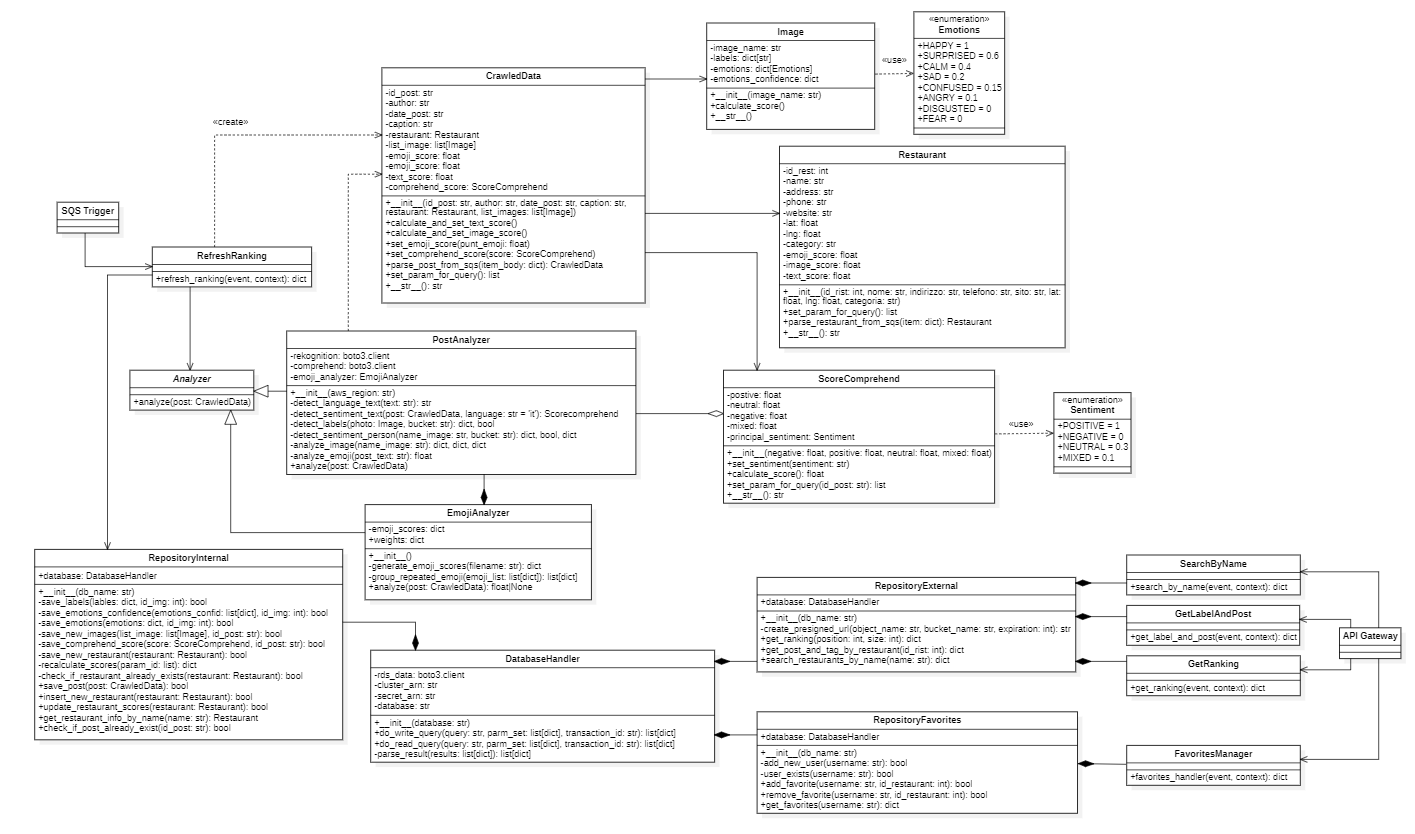
\includegraphics[scale=0.35]{Contenuto/Immagini/classi-RS.jpg}
    \caption{Crawling Service - Diagramma delle classi}
\end{figure}

\subsubsection{Diagrammi di sequenza}
In questa sezione vengono presentati i diagrammi di sequenza che modellano le operazioni principali del Crawling Service:
\begin{itemize}
    \item il suggerimento di un profilo instagram da aggiungere alla lista dei profili su cui viene effettuato il crawling dei dati, nel caso in cui il profilo non sia già presente e sia pubblico;
    \item il processo di crawling dei dati;
    \item la formattazione di un singolo media ottenuto tramite crawling
\end{itemize}
\begin{figure}[H]
    \centering
    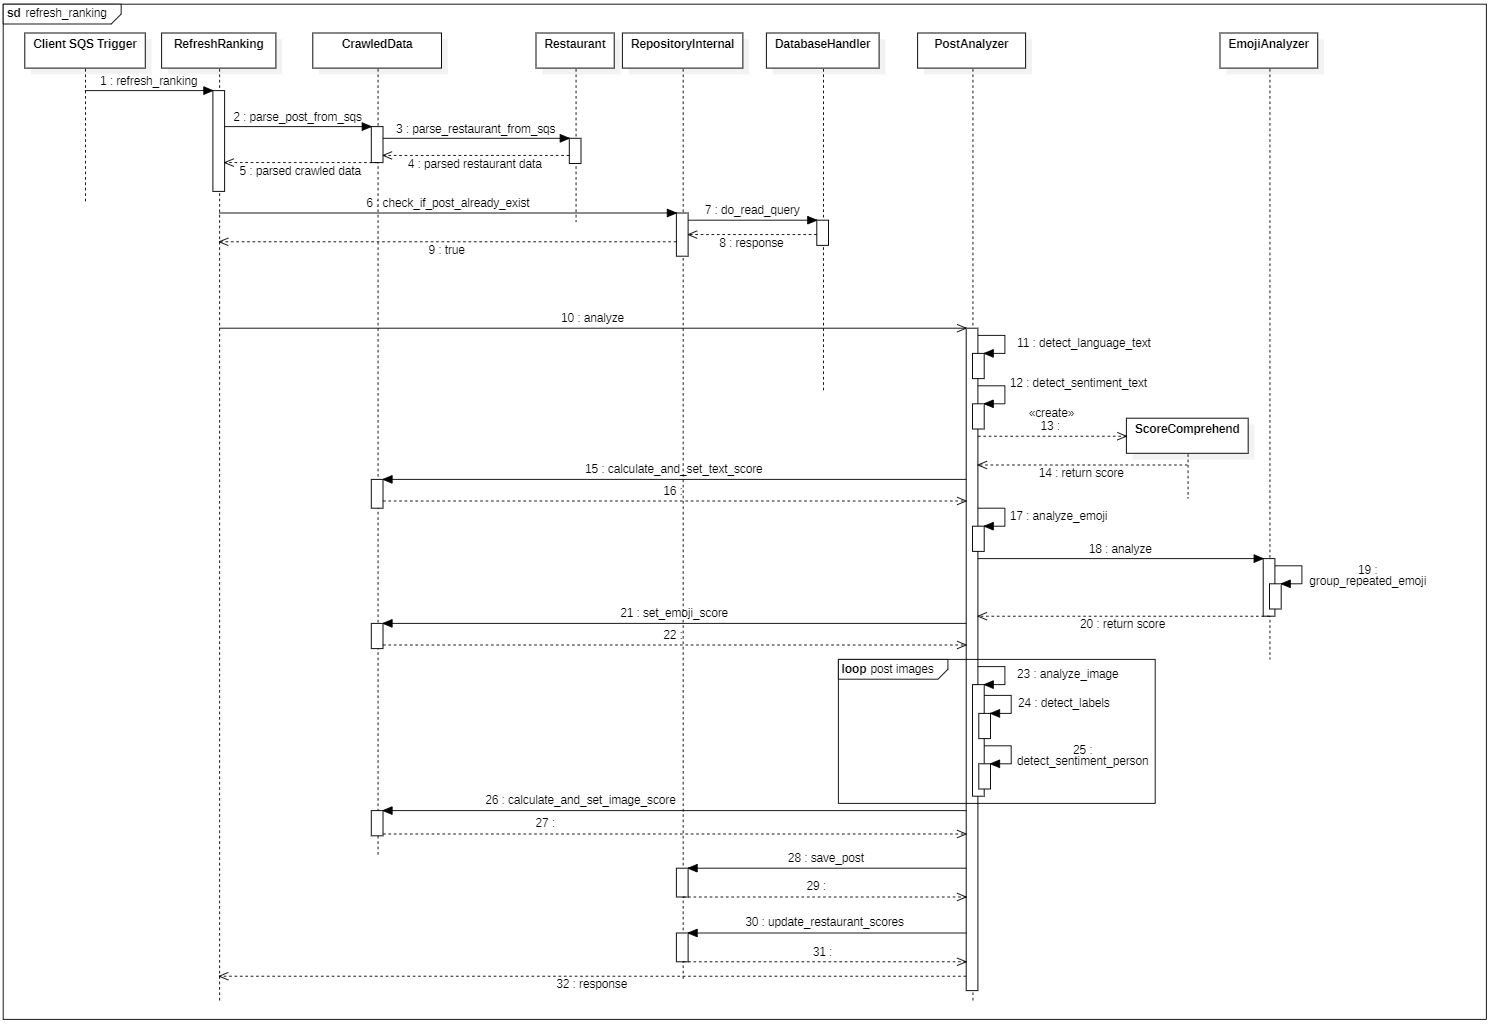
\includegraphics[scale=0.65]{Contenuto/Immagini/seq1-RS.JPG}
    \caption{Crawling Service - Diagramma di sequenza - 1}
\end{figure}
\begin{figure}[H]
    \centering
    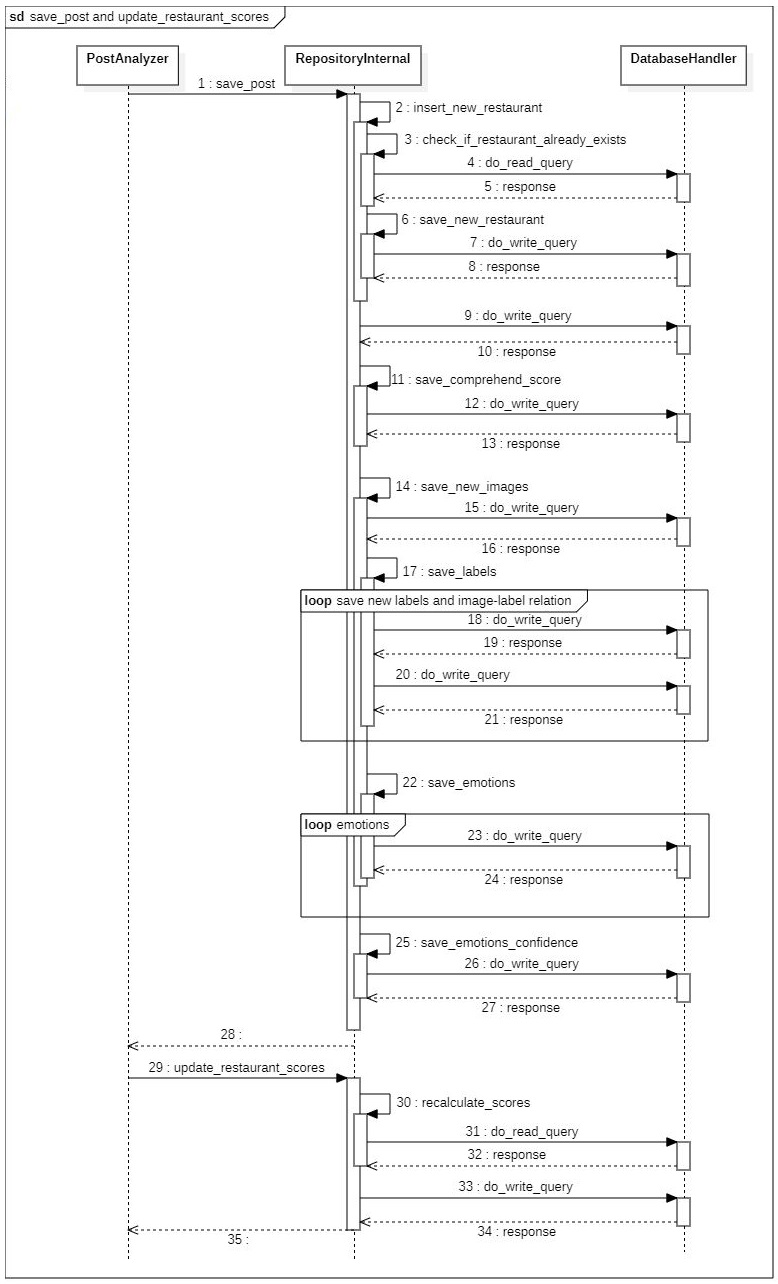
\includegraphics[scale=0.55]{Contenuto/Immagini/seq2-RS.JPG}
    \caption{Crawling Service - Diagramma di sequenza - 2}
\end{figure}


\subsubsection{Design pattern notevoli utilizzati}
Per La realizzazione del Crawling Service sono stati utilizzati i seguenti design pattern:
\begin{itemize}
    \item \textbf{Facade:} Utilizzato per la realizzazione delle classi FacadeCrawling e FacadeAddProfile, in modo da fornire ai client un'interfaccia semplice ad un sottosistema molto complesso e disaccoppiando la logica di implementazione del sistema dal client.
    \item \textbf{Adapter:} Utilizzato dalla classe Crawler pre disaccoppiare il resto del sistema dai metodi di instagrapi, rendendo disponibili solo quelli necessari tramite un'interfaccia nota al sistema.
    \item \textbf{Static Factory:} Utilizzato per fornire dei metodi statici in grado di creare oggetti di tipo CrawledData, Location, ProfileForCrawling a partire da altri tipi di oggetti.
\end{itemize}

\subsubsection{Schema del database}
\begin{figure}[h]
    \centering
    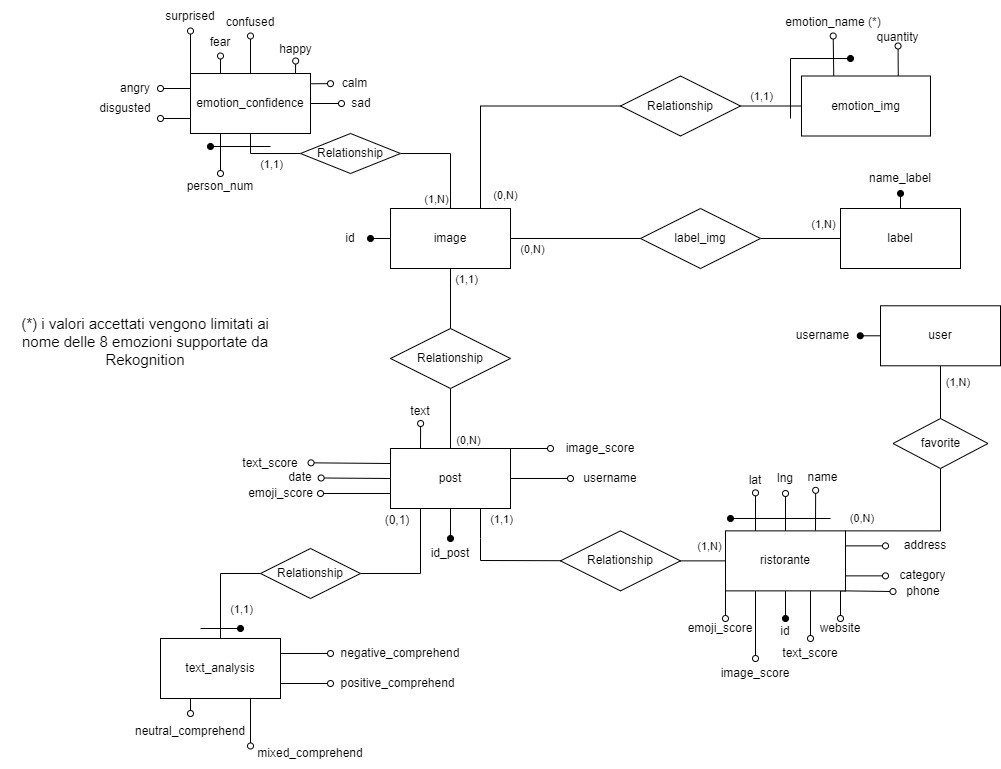
\includegraphics[scale=0.35]{Contenuto/Immagini/ER-RS.jpg}
    \caption{Crawling Service - Schema ER del database}
\end{figure}